\documentclass[10pt,oneside,english,a4paper]{article}
\usepackage[english]{babel}
\usepackage[IL2]{fontenc}
\usepackage[utf8]{inputenc}
\usepackage{graphicx}
\usepackage{url} 
\usepackage{hyperref} 
\usepackage{cite}
\usepackage{listings}
\usepackage[margin=2.75cm]{geometry}

\pagestyle{headings}

\title{How Online Maps Search Works: Technologies, Algorithms and Internal Structure.
\thanks{Semester project in the subject Methods of engineering work, academic year 2023/24, leadership: PaedDr. Pavol Batalik}}

\author{Anton Dmitriev\\[2pt]
	{\small Slovak University of Technology in Bratislava}\\
	{\small Faculty of Informatics and Information Technologies}\\
	{\small \texttt{xdmitriev@stuba.sk}}
	}

\date{\small \today} 



\begin{document}

\maketitle

\begin{abstract}
	Modern online maps have become an integral part of our daily life, providing us with quick access to geographical information and real-time location. However, behind this wonderful opportunity lies a technically complicated system that has been developing and improving for many years. This article provides an overview of the historical and technological development of online mapping and aims to provide an understanding of how modern online maps function and how they provide users with the data they need. Readers will learn how the evolution of technologies in map data has led to the ability to quickly and accurately find places and addresses on a map. Because, in an era where mobile devices and apps are becoming an essential part of our lives, it is important to understand how these maps collect and store information about the world around us, and how they help us navigate and find the places we need.
\end{abstract}

\section{Introduction}
Since the beginning of exploration of our still undiscovered planet Earth, people have worked hard to record the geographical details of the terrain and the routes of their travels. They did this in order to store information that could be used to further improve navigation (More about the History of Cartography in Part ~\ref{history:brief}). The map became a convenient tool for such tasks. However, creating even a single map was a slow and labor-intensive process for the human capabilities of that time. Digital maps, thanks to the ever-increasing availability of computing power, have opened up entirely new possibilities in the field of cartography. Now, after going through this arduous journey of improvements and transformations, a click of the mouse is enough for a computer to plot a user's route from point A to a given point B. "Digital mapping - from the global positioning system (GPS) in your car to the Web site that displays local bus routes - is on the rise" - \cite{Mitchell2005}.
\\The Internet, which has become a source for the development of new technologies, provides the average user with just a convenient online map interface. However, not everyone realizes that behind this attractive skin there is a complex mechanism consisting of many interacting high-tech and modern solutions, designed for easy search by geographical data (More about this mechanism in Part~\ref{internal}).

\paragraph{Reaction to the Social Context Topic:}
Today, online maps play a huge role in the social life of modern humans and, in my opinion, have a significant impact on our sense of the world around us. On the one hand, they have surely brought enormous benefits. Online maps simplify our navigation in unknown places, helping us to find the nearest places we need. By doing this, they increase our mobility and comfort in our daily lives, which is definitely a plus. In addition, online maps boost tourism and travel by providing information about sights and places of interest, making our adventures more exciting and informative. 
\\On the other hand, with the increasing addiction to online maps, we risk losing our navigational skills and sensory perception of the environment. This, as I see it, could lead to a decrease in our ability to navigate the world without the use of technology. In addition, privacy and security of location data are still relevant issues and care must be taken when providing our location, because the constant revealing of this information could make potential risks to personal safety and data privacy. Therefore, despite the obvious benefits of online maps, I believe that we need to use these services wisely and when it is necessary.

\section{History of Online Maps Development} \label{history}

\subsection{A Brief Background in Cartography} \label{history:brief}
In order to understand modern online maps, it is crucial to delve into the historical roots of cartography. Cartography is a captivating blend of science and art, endeavoring to depict the world as accurately as possible while grappling with the challenge of what to include or leave out. This challenge pertains not only to geographical features but also extends to the selection of a map projection, a pivotal aspect in transforming the spherical Earth into a flat map.
\\Early cartography involved the creation of maps that primarily served navigational purposes. For instance, Polynesian and Micronesian voyagers crafted intricate stick charts to map connections between islands and interpret swell patterns. Portuguese explorers, on the other hand, produced detailed coastal maps that often left the interiors largely blank since their focus was on exploration and seafaring.
\\In 1569, Flemish cartographer Gerardus Mercator introduced a revolutionary map projection\cite{Forrest2021}, which was designed to assist sailors in plotting a straight-line course between any two points. The Mercator projection, or variations thereof, remains the dominant choice in online mapping today due to its ability to depict the entire globe on a nearly square image. However, it comes with a trade-off, introducing size distortions, making it appear as if Greenland is comparable in size to the entire African continent, when in reality, Africa is roughly 14 times larger than Greenland (Figure~\ref{fig:mercator}).

\begin{figure}[h]
	\centering
	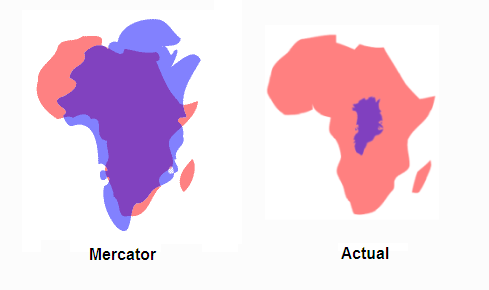
\includegraphics[scale=0.5]{diagram4.png}
	\caption{Difference between Mercator Projection and Reality \cite{Forrest2021}}
	\label{fig:mercator}
\end{figure}

\subsection{The First Maps on the Web} \label{history:firstweb}
The emergence of online mapping can be traced back to the early days of the internet. While pinpointing the very first online map is challenging, the transition from static map images to interactive web maps marked a significant milestone. Interactive web maps empowered users, allowing them to control their exploration—zooming in and out, toggling map layers, and more.
\\One of the earliest web maps, the PARC Map Viewer, made its debut in 1993, thanks to Xerox. This pioneering map viewer allowed users to view maps, interact with map features, and toggle map layers \cite{Forrest2021}. Fundamentally, it operated on a straightforward principle: a user requested a map, the viewer fetched data from a geographic database, rendered a map image, and transmitted it back to the user's browser. This fundamental request-render-return loop remains the core of most web maps today.
\\The PARC Map Viewer was also instrumental in the inception of "mashups." It allowed overlaying data on maps, exemplified by the display of earthquake data facilitated by the World-Wide Earthquake Locator developed by the University of Edinburgh in 1994. This mashup concept gained swift adoption among developers, heralding a new era in web mapping (More about "Mashups" in Part~\ref{history:mashups}).

\subsection{The Rise of Consumer-Facing Web Mapping Services} \label{history:userfriendly}
In 1996, Mapquest and Multimap, both launched in the same year, marked the advent of user-focused web mapping services. These platforms offered users the ability to input their addresses and witness their locations represented on maps, which was a revolutionary concept at the time. Mapquest, in particular, introduced features like zooming and panning, enhancing the interactivity of web maps \cite{Forrest2021}.
\\User-friendly web mapping services revolutionized navigation by rendering traditional printed road maps increasingly obsolete. The ease of locating oneself and obtaining driving directions online fundamentally reshaped how people navigated the world around them.
\\However, these early web maps had a limitation: every time the map was panned or zoomed, the entire map view had to reload, resulting in a somewhat slow user experience.

\subsection{Google Maps: A Game-Changer} \label{history:gamechanger}
Google entered the web mapping arena and turned the tables in 2005 with the launch of Google Maps \cite{Forrest2021}. Google Maps incorporated groundbreaking features like satellite imagery and an interactive interface, which garnered rapid popularity. 
\\Key to the success of Google Maps was its use of map tiles, small square images that made up the larger map, and the utilization of the Mercator projection~\ref{history:brief}. These tiles allowed for faster loading times and efficient use of resources. Moreover, Google's innovative map tiles were capable of rendering different zoom levels, further enhancing the user experience~\ref{data:types}. 

\begin{figure}[h]
	\centering
	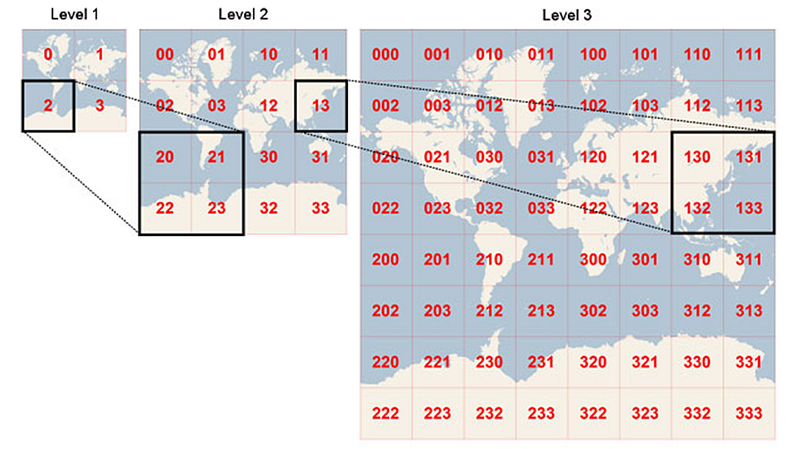
\includegraphics[scale=0.35]{diagram5.png}
	\caption{Map Tiles at Different Zoom Levels \cite{Forrest2021}}
	\label{fig:tiles}
\end{figure}

Google Maps didn't stop at providing directions but went a step further by introducing a blue dot to indicate a user's precise location (Due to Location Positioning Technologies ~\ref{internal:gps}). This feature opened the door to a new industry centered around location, with services like Foursquare and Yelp leveraging location data for various purposes, from reviews to recommendations.

\subsection{Terravision: A Pioneering 3D World Mapping Software} \label{history:patentrights}
It would seem that we all know the most popular online mapping service such as Google Maps (originally Google Earth). But there were some dark places in its history of creation. Terravision\cite{Leclerc1994} was a one of the firs 3D world mapping software program developed by a group of German university students from ART+COM, including Jachim Sauter and Juri Muller. Launched in 1993, Terravision aimed to provide a networked, virtual, and graphical representation of Earth using 3D graphics. Juri Muller, as the chief programmer, was responsible for inventing the algorithms that powered the software. Joachim Sauter, on the other hand, focused on the program's design and artistic elements. The result was a unique fusion of art and technology.
\\Terravision quickly gained worldwide attention in the early '90s, as it was a novel concept not seen in the technology and internet landscape of that time. During the exhibition tours, the creators of Terravision made a visit to Silicon Valley, where Juri Muller accidentally told the details of Terravision's algorithms to Brian McClendon, an American software engineer and skilled programmer.Brian used this information to develop in collaboration with Google a program that would later become a household name in the field of online mapping, "Google Earth".
\\In 2014, ART+COM, the company responsible for Terravision, filed a lawsuit against Google, alleging that Google's product, Google Earth, infringed upon the patent rights of Terravision, which had been invented in 1993. Two years later, the legal dispute reached its resolution: The United States District Court for the District of Delaware ruled in favor of Google \cite{ArtcomGoogle2017}.
\\The legal clash between Terravision and Google attracted significant attention and ultimately became the subject of a Netflix series titled "The Billion Dollar Code."

\subsection{Mashups and the Emergence of OpenStreetMap} \label{history:mashups}
While Google Maps was gaining momentum, developers were beginning to explore the idea of integrating their own data into web maps. This was exemplified by Paul Rademacher, who ingeniously used unsanctioned APIs from Google Maps to create HousingMaps.com, a platform that combined Craigslist rental listings with Google Maps. This represented the birth of mashup mapping, which allowed users to overlay their data onto established web map services.
\\Instead of shutting down these mashups, Google embraced the trend by introducing the Google Maps API, which made it possible for developers to utilize Google Maps as a service for their applications \cite{Forrest2021}. This step effectively commercialized the mapping product.
\\The idea of overlaying data on web maps and the popularity of Google Maps inspired a new generation of mapping services and projects. Notably, OpenStreetMap (OSM) , launched in 2004, gained traction by inviting users to add or edit map features, such as roads, waterways, and points of interest. OSM, often described as the "Wikipedia for maps," fostered a global community of contributors, leading to a significant increase in data quality and coverage.

\subsection{Vector Tiles and the Democratization of Mapping Data} \label{history:vector}
The transformation of web maps continued with the introduction of vector tiles (Figure~\ref{fig:vector}), a significant leap forward in technology. Unlike traditional map tiles that consist of static images, vector tiles contain raw geospatial data that can be rendered in real-time by the browser. This shift made maps more dynamic, allowing for smoother and more interactive map experiences.
\\Vector tiles were especially well-suited for the mobile environment and were made possible through technologies like WebGL, which enhanced graphics rendering in browsers \cite{Forrest2021}. This innovation allowed developers to create map-based applications with greater efficiency and flexibility.
\\Web mapping saw a pivotal moment when Uber sought to visualize its extensive ride data. Faced with vast amounts of ride records, Uber embarked on the development of tools that could efficiently handle and visually represent massive datasets. One of the outcomes was Deck.gl, a framework for rendering large-scale data visualizations on maps. This open-source project opened doors for data visualization in various fields, from urban planning to spatial analytics.

\paragraph{Reaction to the Historical Context Topic:}
Online maps are, in my opinion, an amazing tool for visualizing geographic information, and the historical context of their development is very interesting. When I started researching this topic, I learned that it has a long history, starting with ancient cartography and Mercator maps. This shows for how long people have been aiming to represent the world in a cartographic format and are still moving towards more and more accurate representations of our globe.
\\However, the real revolution has come with the development of online maps as a result of the digital revolution. With the advent of the internet and computer technology, it has become possible to access geographical information easily and quickly. This has made navigation, research and route planning much easier, making the world more accessible and understandable for everyone. I believe that this highlights the importance of technological advances in this field and shows the effort to make geographical data more accessible and convenient for everyone.


\section{Internal Structure} \label{internal}

\subsection{Shortest Path from Point A to Point B} \label{internal:dijikstra}
Google Maps utilizes graph data structures to compute the shortest route from a source point (point A) to a destination (point B). A graph data structure is composed of numerous nodes interconnected by multiple edges. Edsger W. Dijkstra introduced the Dijkstra's algorithm, an efficient method for determining the shortest distance and path to a specified destination. In this graph, nodes are linked by weighted edges, which signify the distance required to travel to each node. 
\\Here's how this algorithm works\cite{Mehta2019}:

\begin{enumerate}
	\item Choose an initial node in the weighted graph which serves as a source node.
	\item The distance of the other nodes is intialised as infinity with respect to the source node. 
	\item An empty set N containns the nodes to which the shortest path has been found. 
	\item The distance of the source node with respect to itself is zero. It is added to N and thus termed as ‘active node’. 
	\item Consider the neighbouring nodes of the active node which are connected to it by a weighted edge. Sum up the distance with the weight of the edge. 
	\item If the neighbouring nodes already have some distnace assigned, then update the distance if the newly obtained distance in step 5 is less than the current value. 
	\item Now, choose the node which has the minimum distance assigned to it and insert it into N. The newly inserted node is now the ’active node’. 
	\item Repeat steps 5 to 7 until the destination node is included in the set N or if there are no more labelled nodes in N.
	
\end{enumerate}

\begin{lstlisting}[language=C++, caption=Pseudo code representation, frame =single, basicstyle=\ttfamily\small]
function  dijkstraAlgorithm(graph, source):
	for each node n in graph:
		distance[n] := infinity
		previous[n] := undefined
	distance[source] := 0
	q := the set of all nodes in graph
	while q is not empty:
		z := node in q with smallest distance[ ]
		remove z from q
		for each unvisited neighbor n of z:
			dist := distance[u] + dist_between(z, n)
			if dist < distance[n]
				distance[n] := dist
				previous[n] := z
return distance[ ] previous[ ]

\end{lstlisting}
In the context of Google Maps, this graph represents the road network, with each road segment serving as a node and intersections as the connecting points. While the Dijkstra's algorithm may lose its efficiency when dealing with the big data of Google Maps, it still forms the foundational concept of the algorithm that modern online maps rely upon to determine the shortest path between two points.

\subsection{What is Geocoding?} \label{internal:geocoding}
Geocoding is a fundamental component of spatial analysis that has found applications across various research disciplines and domains. It involves the process of converting descriptive locational data, such as postal addresses or named places, into absolute geographic references. Over the years, geocoding has undergone significant evolution, transforming from a costly and limited practice to a more accessible and accurate method, often available for free through online services \cite{Goldberg2007}. 
\\Early geocoding systems, like those used by the U.S. Census in the 1960s, primarily assigned numerical codes to postal addresses and named buildings, resulting in low-resolution geographic output. Then the idea of geocoding was extended in the early 20th century with the development of automobile navigation systems. The main challenge was to develop a way to convert textual descriptions of addresses (e.g., "1010 E Main St, Waynesboro, VA 22980, USA ") into numerical coordinates (38.064050, -78.873830) that could be used for navigation. This first became widely available through the Global Positioning System (GPS) in the late 20th century.
\\Geocoding is based on mapping text addresses to geographic coordinates (Figure~\ref{fig:geocoding}). The process involves the following steps \cite{Behr2010}:

\begin{enumerate}
\item \textbf{Receiving the request} - user enters a textual description of the location into the search box or through the map interface.
\item \textbf{Analyzing the query} - server analyzes the request, trying to understand what type of location is specified (e.g., address, place name, zip code, etc.).
\item \textbf{Database Search} - server accesses its geographic database, which contains information about millions of locations. It looks for a match between the query entered and the data in the database.
\item \textbf{Result ranking} - server returns a list of the most likely results ranked by similarity to the request. 
\item \textbf{Geographic coordinates output} - The server returns the geographic coordinates (latitude and longitude) of the selected location.
\item \textbf{Display on map} - received coordinates are used to display the selected location on the map. The map is centered on that location and information about the location is shown to the user.
\end{enumerate}

\begin{figure}[h]
	\centering
	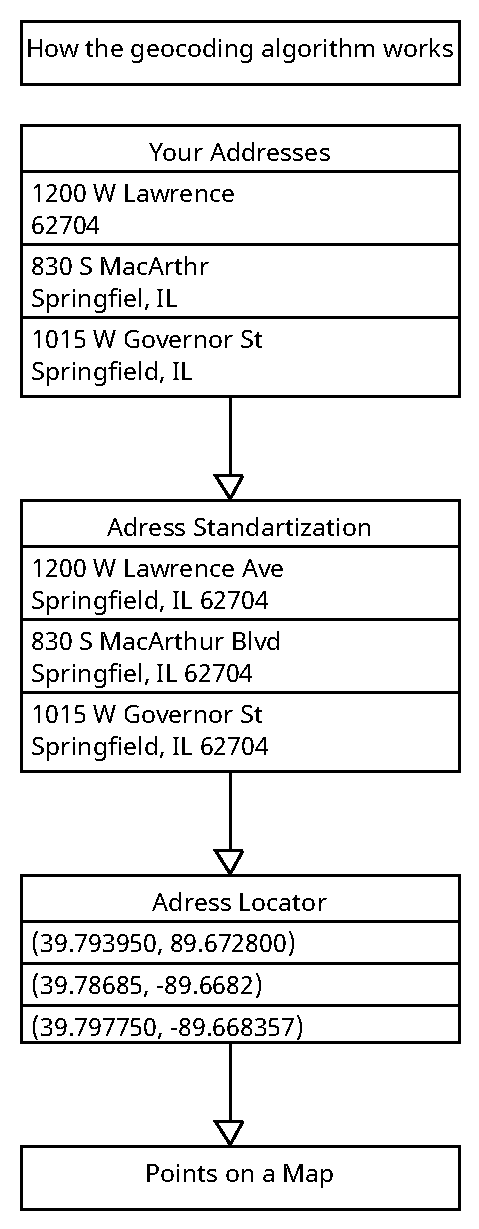
\includegraphics[scale=0.45]{diagram1.pdf}
	\caption{Process of Geocoding}
	\label{fig:geocoding}
\end{figure}

So modern online maps make extensive use of geocoding to provide location information and navigation. Here are a few scenarios of how geocoding is used in modern online maps:

\begin{itemize}
\item \textbf{Searching and finding places:} Geocoding allows online map users to find places by address or keywords. A user can type in the name of a restaurant, store, or address, and online maps will convert that query into coordinates and display the location on the map.
\item \textbf{Navigation and route creation:} When creating routes between two points, geocoding is used to determine the coordinates of the start and end points and to find the best route between them.
\item \textbf{Information about nearby objects:} Maps use geocoding to provide information about nearby objects such as restaurants, hotels, gas stations, and other establishments. The user can see their location on the map and get more information about them.
\item \textbf{Geotagging of photos:} If a user takes a photo of a location using a mobile device, the phone can use geocoding to automatically add location coordinates to the photo. This allows users to organize and find photos by location.
\end{itemize}

Geocoding plays an important role in the functionality of modern online maps, making it a powerful tool for navigating, finding places, and getting information about geographic locations. Accurate geocoding can greatly enrich the user experience and help find information about the world around them. 

\subsection{Location Detection: You Can't Hide from It} \label{internal:gps}
Global Positioning System (GPS) - is an U.S. Government-owned satellite utility that provides users with positioning, navigation, and timing services\cite{GPS.gov}.
\\The idea of GPS originated in the second half of the 20th century. In 1957, the USSR launched the first artificial satellite, which was the beginning of the space age. This inspired the US to develop a satellite navigation system. The GPS development project began in 1973 when the US announced a global navigation system. The first GPS satellite was launched in 1978 and the system was operational within a few years.
\\GPS was originally developed for military purposes to provide accurate positioning and navigation for the armed forces. Thereafter, access to the system was opened up for civilian use. As the system began to be opened up for civilian use, GPS became an integral part of everyday life. It is used for navigation on roads, in aviation, maritime, and in geopositioning-related applications and websites, such as online maps.
\\GPS is based on the idea of triangulating a point in space. To determine the position of a point in space, it is sufficient to know the distance from it to three other points with known coordinates. In geodesy and radio communications, this is called triangulation - when we can use the coordinates of three points to calculate where the fourth (our) point is. In mobile phones without a GPS module, it works like this (Figure~\ref{fig:triangulation}):

\begin{enumerate}
\item The mobile phone picks up signals from three radio communication towers.
\item These signals transmit, among other things, the coordinates of the towers themselves.
\item The mobile phone measures the time it takes for the signal to reach each tower.
\item Based on this time, it calculates the coordinates of its location with an accuracy of 10-20 meters.
\end{enumerate}

\begin{figure}[h]
	\centering
	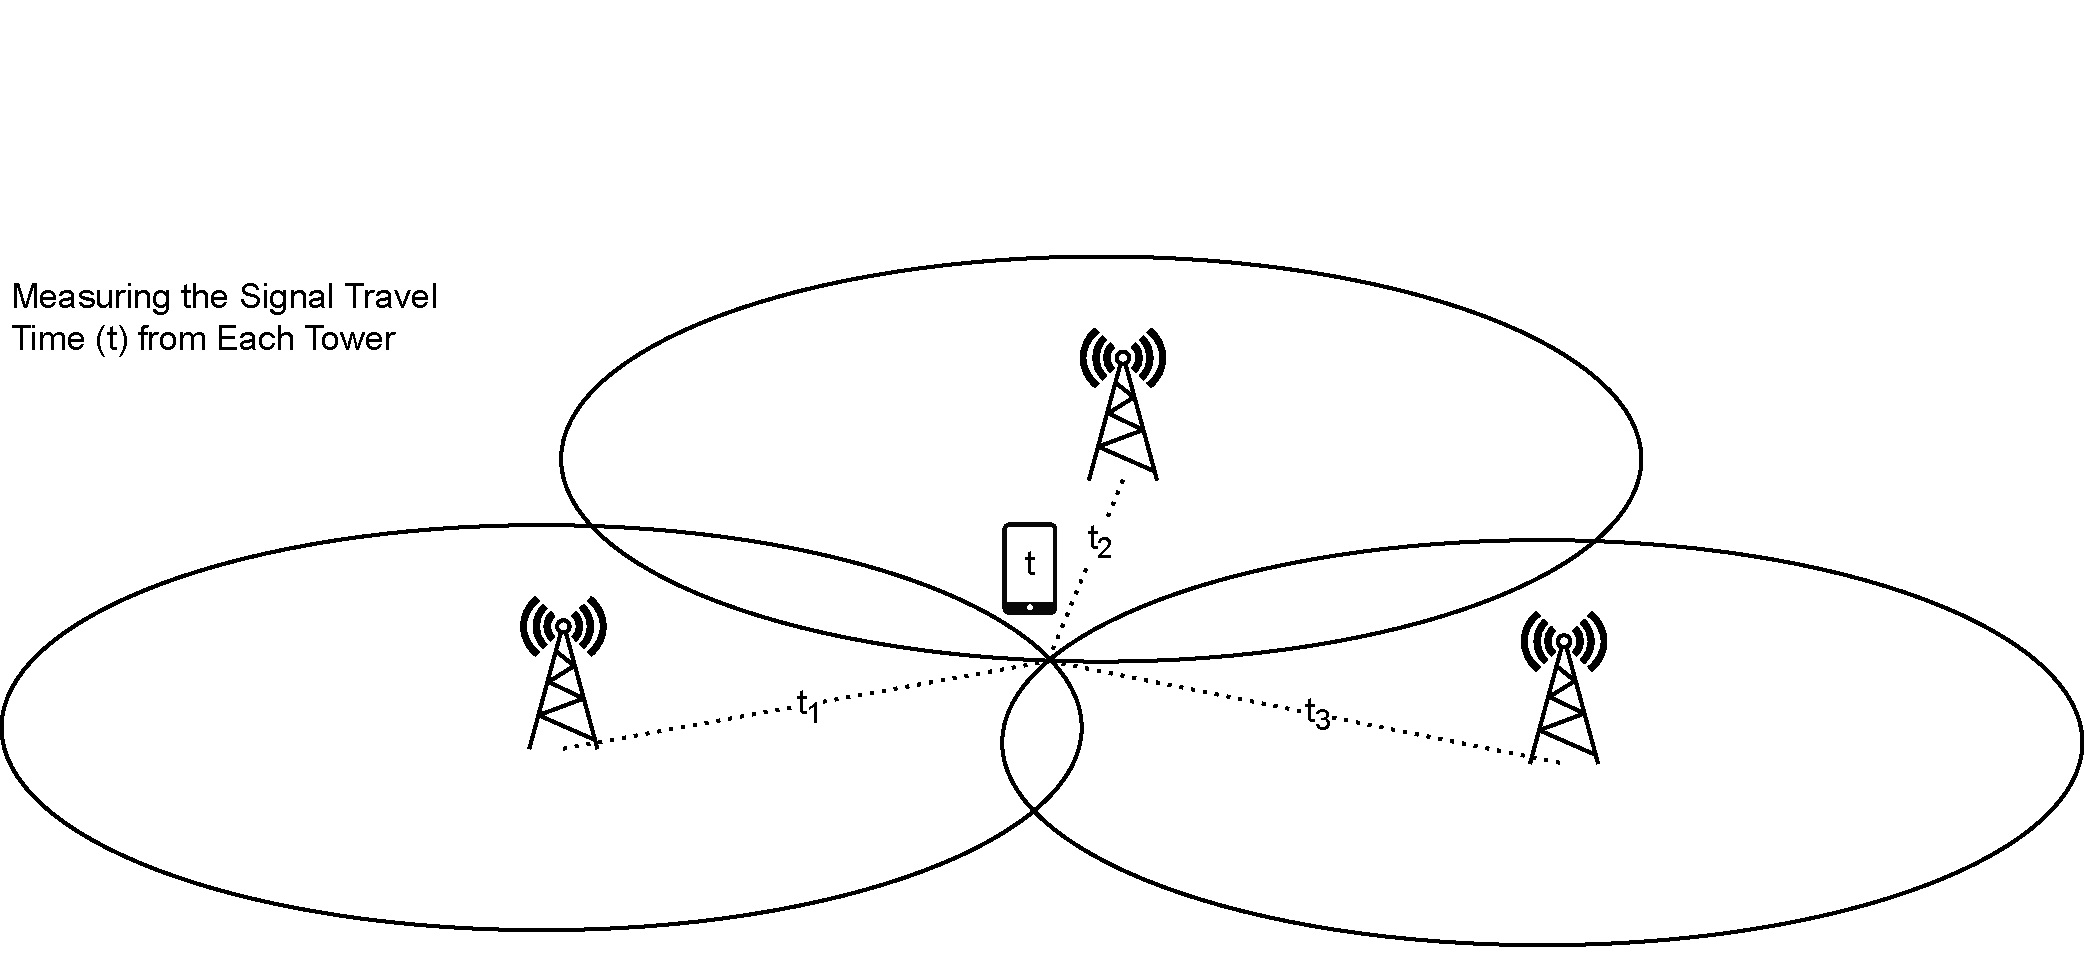
\includegraphics[scale=0.3]{diagram2.pdf}
	\caption{Visual Example of Triangulation}
	\label{fig:triangulation}
\end{figure}

Now that we know the basic idea, we move to satellites. In GPS positioning, instead of communication towers there are satellites. The task of such a satellite is to constantly transmit its coordinates, time information and other service data to the ground. All this is sent from the satellite in the form of radio signals at a frequency of about 1.5 gigahertz at a rate of 50 bits per second. Constantly and 24 hours a day, 7 days a week. To calculate the exact distance to the satellite, you need to measure the signal travel time very accurately. To do this, an atomic clock is placed in each satellite that transmits time with an accuracy of 10$^{-11}$ seconds. This allows you to calculate the position of each satellite with an accuracy of a few meters. 
\\For the work of GPS in phones is responsible for a separate radio module - it is tuned to the frequencies of satellites, and it has all the necessary algorithms for calculations. And now we can use the logic of triangulation, which in the case of satellites is called trilateration\cite{Bajaj2002}:

\begin{enumerate}
\item The phone gets a signal from the first satellite, but that doesn't give it anything.
\item After receiving a signal from the second satellite, the phone realizes the approximate circle in which it is located. The circle can be a hundred kilometers in diameter, so there are no exact coordinates yet.
\item After the signal from the third satellite, the phone can calculate the approximate location with an accuracy of about 10 meters (Figure~\ref{fig:trilateration}).
\item But after the signal from the fourth and all subsequent satellites - with an accuracy of one meter.
\end{enumerate}

\begin{figure}[h]
	\centering
	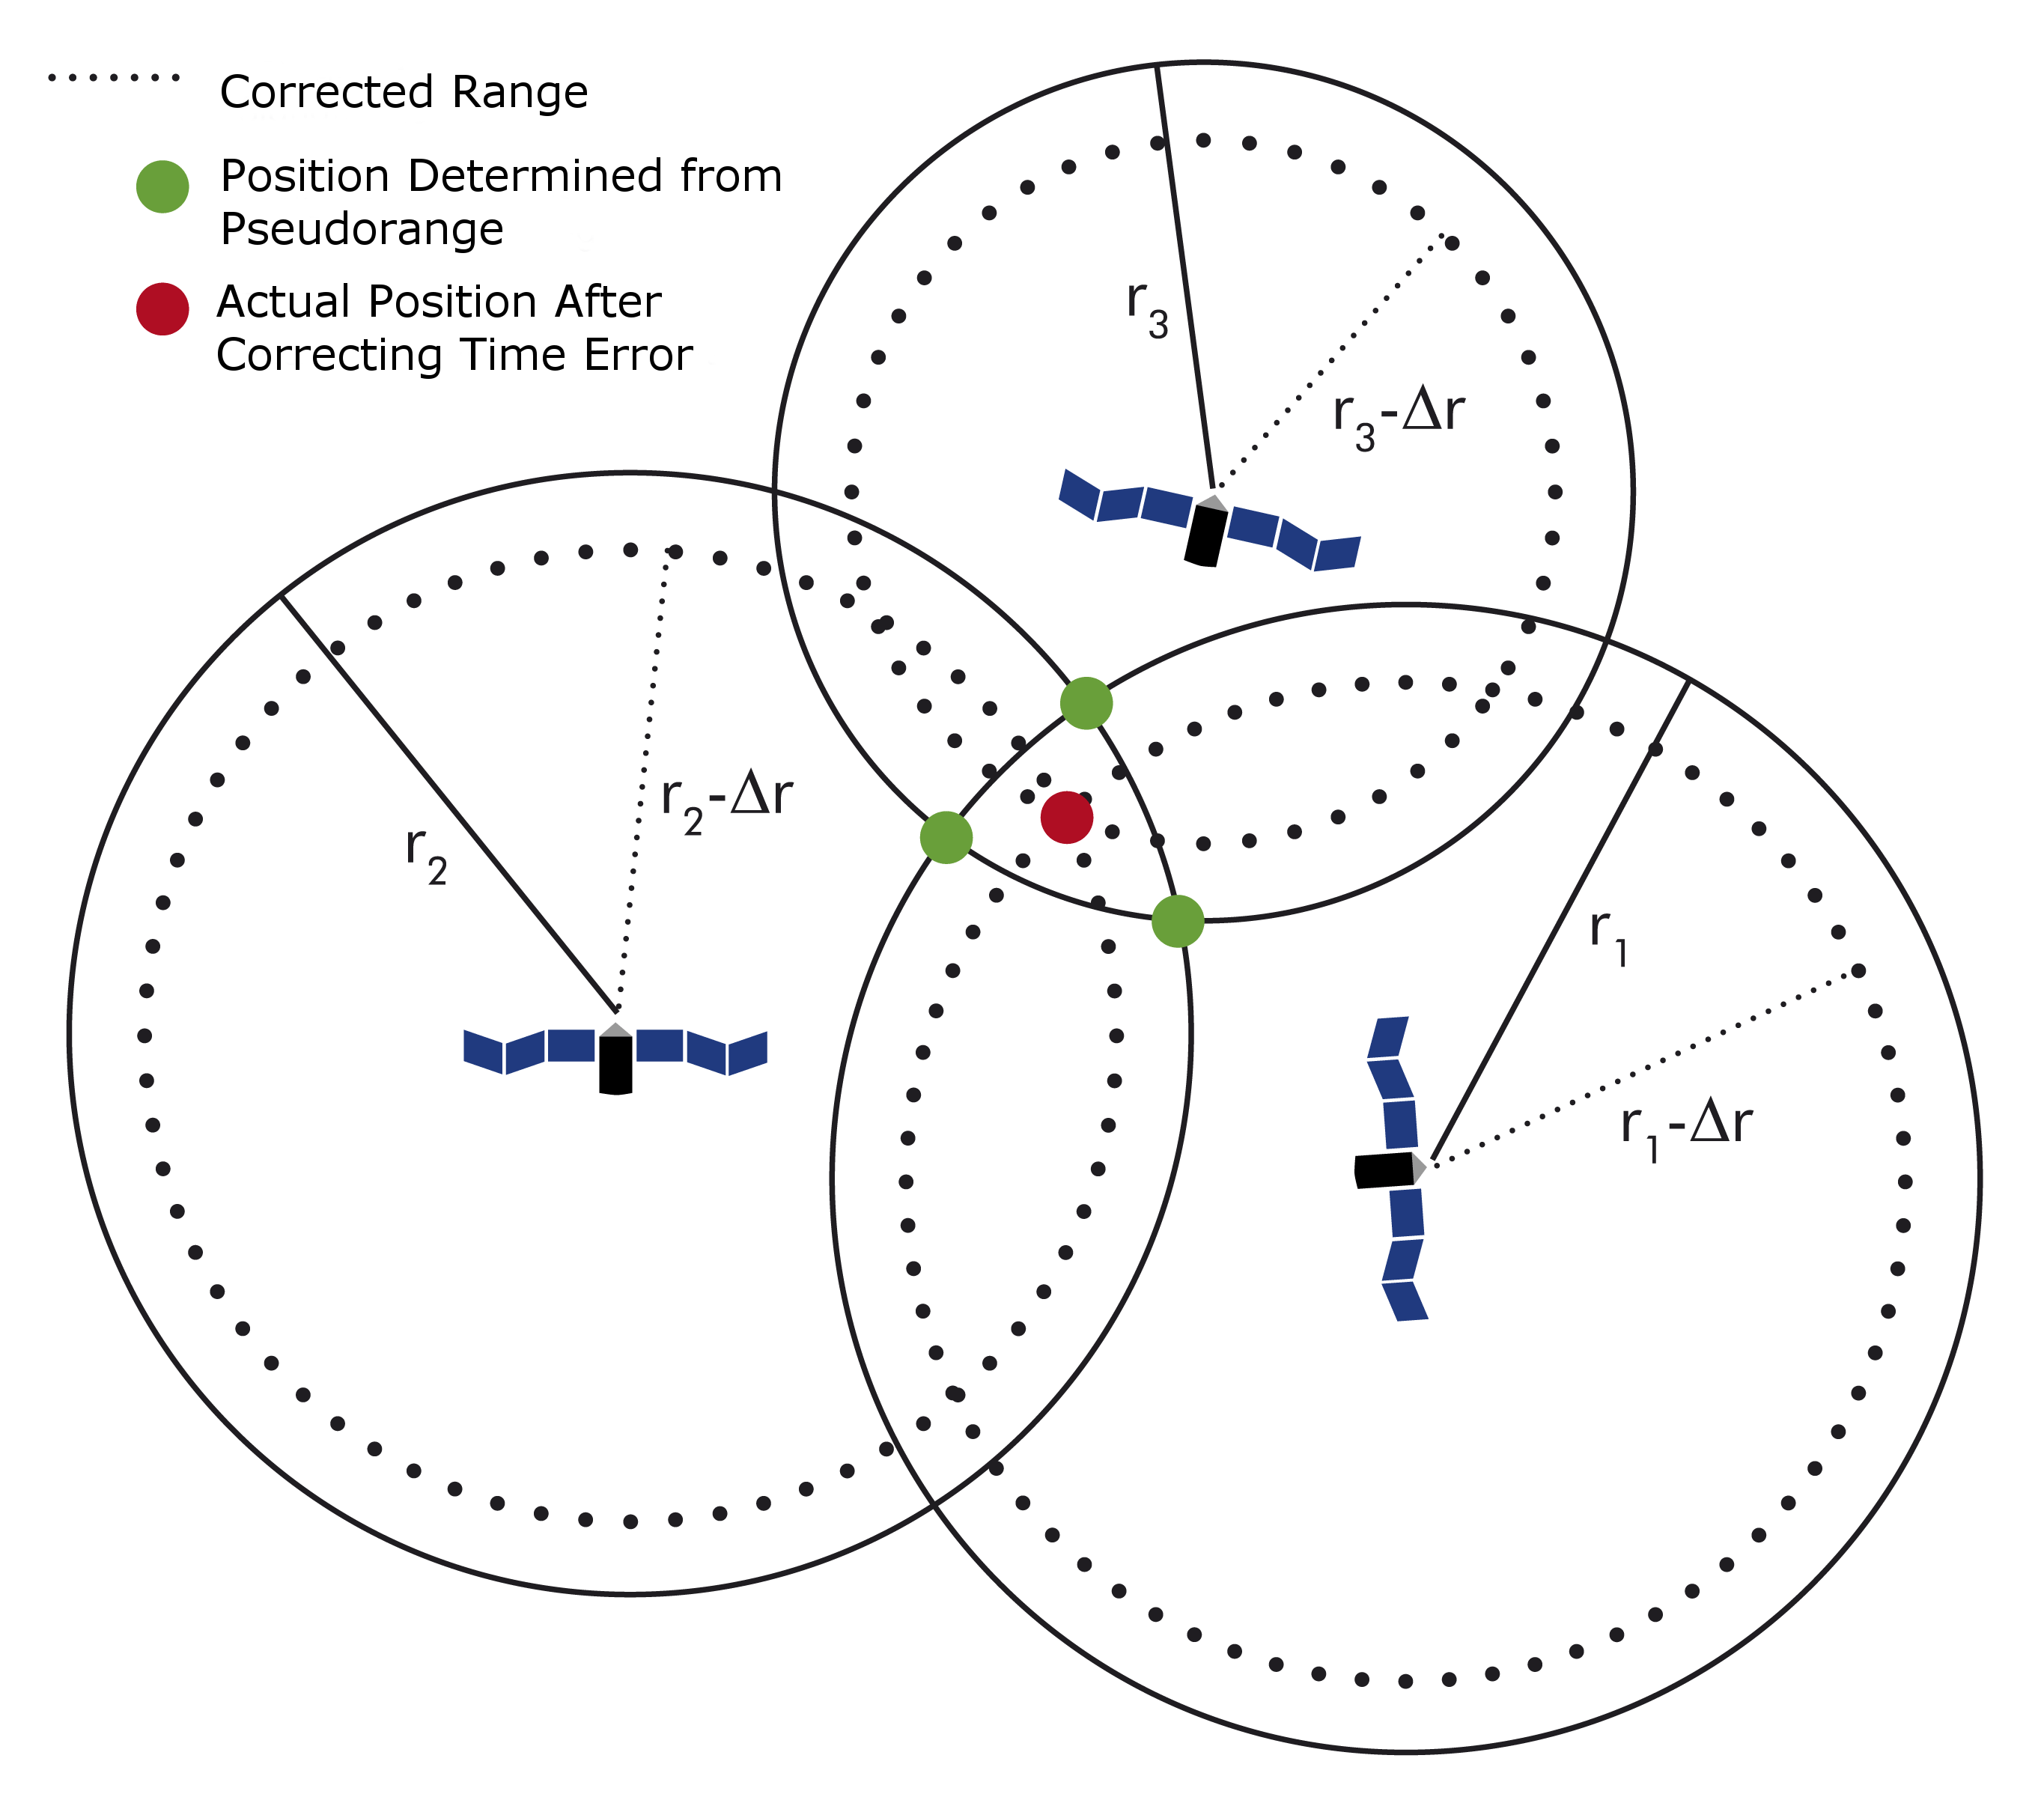
\includegraphics[scale=0.07]{diagram3.png}
	\caption{Visual Example of a 3-satellite GPS Trilateration \cite{Olson2018}}
	\label{fig:trilateration}
\end{figure}

GPS - the first, but not the only global positioning system. Now there are three more such systems of this level working in the world. They have different operating frequencies, but the same principle of operation:

\begin{itemize}
\item \textbf{GLONASS} is a Russian system with 27 satellites (GPS has 32). It has higher accuracy than GPS;
\item \textbf{Beidou} - belongs to China, now it includes 15 satellites - this is the minimum number for stable navigation;
\item \textbf{Galileo} - European system, 23 satellites.
\end{itemize}

What system to work with - depends on what module is in the receiver (in the phone or navigator). Now most smartphones support all systems except Galileo, which means that 20-30 satellites can be used for positioning. This does not give an increase in accuracy, but it gives reliability - if the satellites of one system are unavailable, you can navigate by the others. As a result, GPS is integrated into online maps to provide users with accurate and convenient interaction with location and navigation data, making the use of maps in everyday life more convenient and efficient.

\section{Data Structure} \label{data}

\subsection {Geographic Data Management Tool} \label{data:gis}
Geographic Information Systems (GIS) are complex tools that collect, store, process, analyze, and visualize data associated with specific geographic coordinates \cite{LandId2021}. GIS data is not just a collection of information; it is a way of understanding and interpreting landscapes, weather patterns, populations, and other important aspects of an area. In the context of online maps, this data helps in creating detailed, interactive and feature-rich map products.

\subsection {Types of GIS Data} \label{data:types}
GIS data is categorized broadly into two types, each with distinct characteristics and applications\cite{Chang2016}:

\textbf{Raster Data:} This type of data is composed of a grid of cells, or pixels, each representing a specific area on the earth's surface (Figure~\ref{fig:tiles}). These pixels encode information like color, temperature, or elevation. Raster data is integral to satellite imagery and aerial photography, offering a macroscopic view of geographic areas. It is particularly useful in environmental monitoring, urban development analysis, and tracking landscape changes over time.

\textbf{Vector Data:} Vector data, in contrast, uses geometric shapes—points, lines, and polygons—to represent spatial features (Figure~\ref{fig:vector}). This data type excels in depicting discrete elements such as road networks, building outlines, and water bodies. Its precision in detailing exact locations and boundaries makes vector data a critical resource in areas like city planning, transportation infrastructure, and geographic boundary delineation.

\begin{figure}[h]
	\centering
	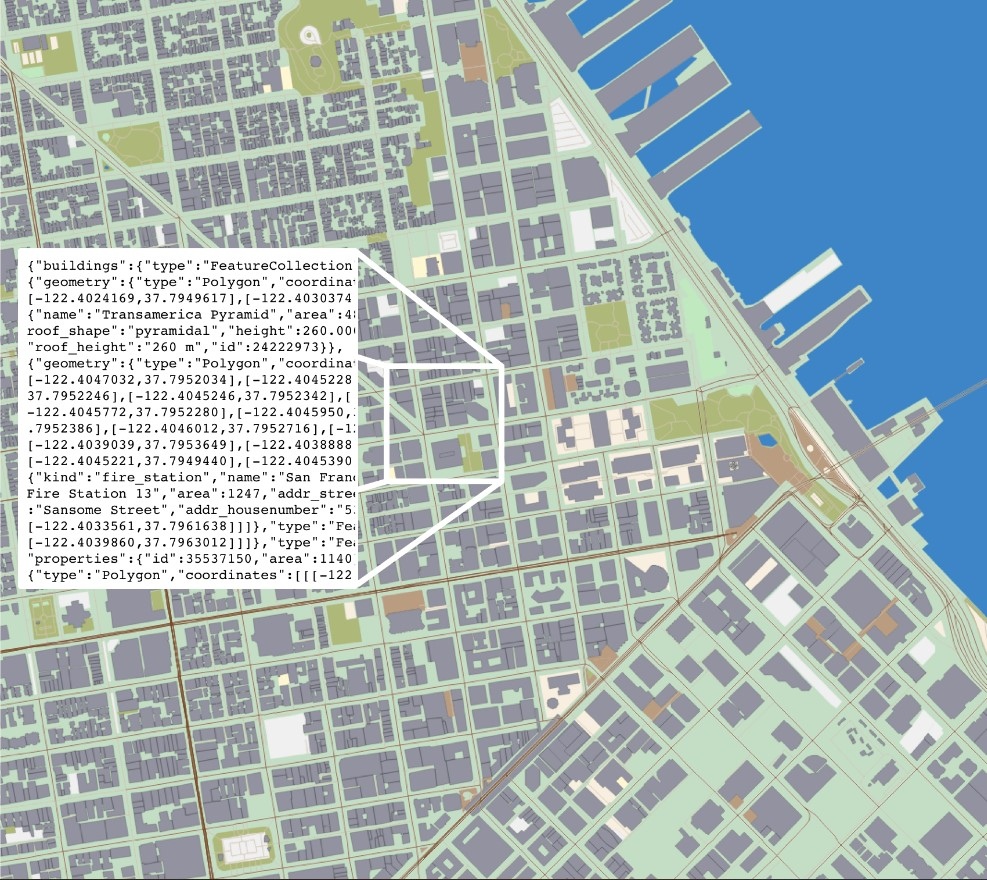
\includegraphics[width=0.45\textwidth]{diagram6a.jpg}
	\hfill
	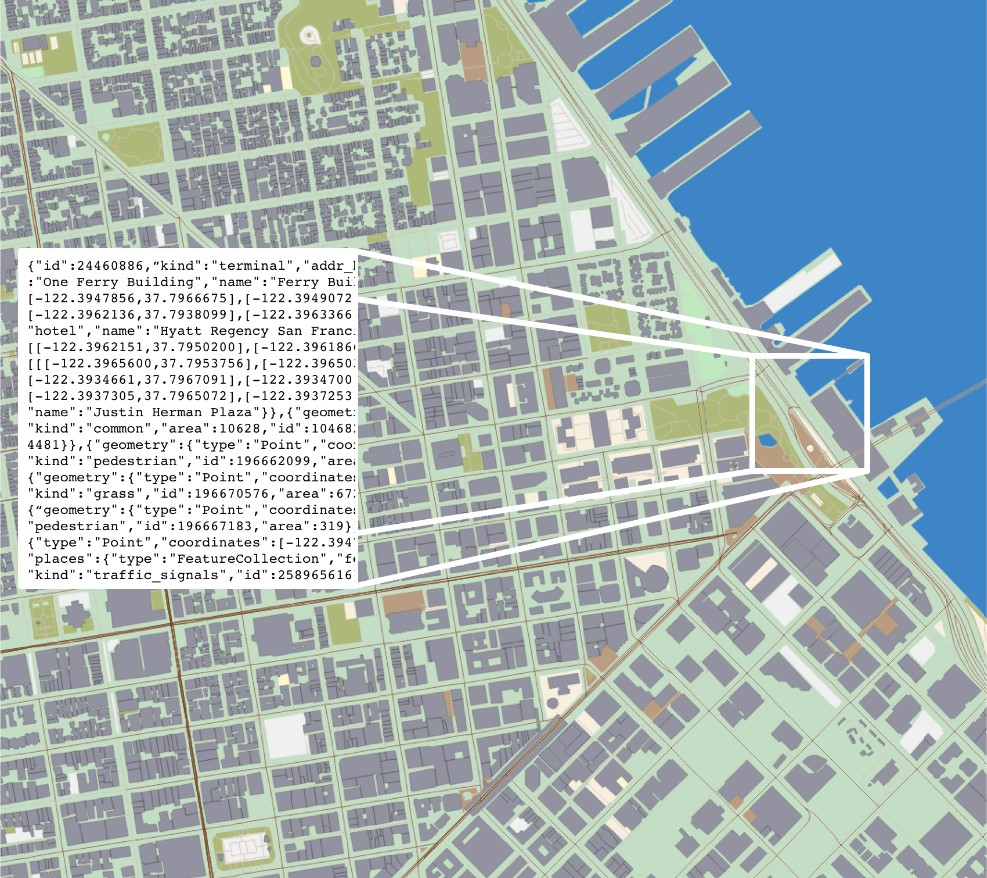
\includegraphics[width=0.45\textwidth]{diagram6b.jpg}
	\caption{Two Different Vector Tiles \cite{Allegri2017}}
	\label{fig:vector}
\end{figure}

\subsection {Methods and Sources of Data Collection} \label{data:sources}

The collection of GIS data employs a variety of methods, each tailored to capture different aspects of spatial information \cite{Demers2008}:

\begin{itemize}
\item \textbf{Remote Sensing:} This involves the acquisition of data from satellite or aerial platforms \cite{Novak1995}. Remote sensing is particularly effective for gathering extensive raster data, providing a wide-angle view of earth’s topography and environmental conditions. It is a key tool in large-scale environmental assessment, climate change studies, and disaster management.

\item \textbf{Aerial Photography:} Capturing high-resolution images from the air, aerial photography is instrumental in creating detailed topographic maps and landscape analyses. It finds applications in agriculture for crop assessment, urban planning, and environmental conservation efforts.

\item \textbf{LiDAR (Light Detection and Ranging):} LiDAR technology (Figure~\ref{fig:lidar}) uses laser pulses to measure distances and generate precise three-dimensional models of the earth's surface. It is highly valued in surveying, forestry management, and infrastructure development, particularly for its accuracy in terrain modeling and elevation assessment.

\item \textbf{Ground Surveys:} Ground surveys provide the highest accuracy for vector data collection, especially for detailed measurements of land parcels, infrastructure, and urban layouts. They are conducted using traditional surveying techniques, measuring angles and distances from established reference points.

\begin{figure}[h]
	\centering
	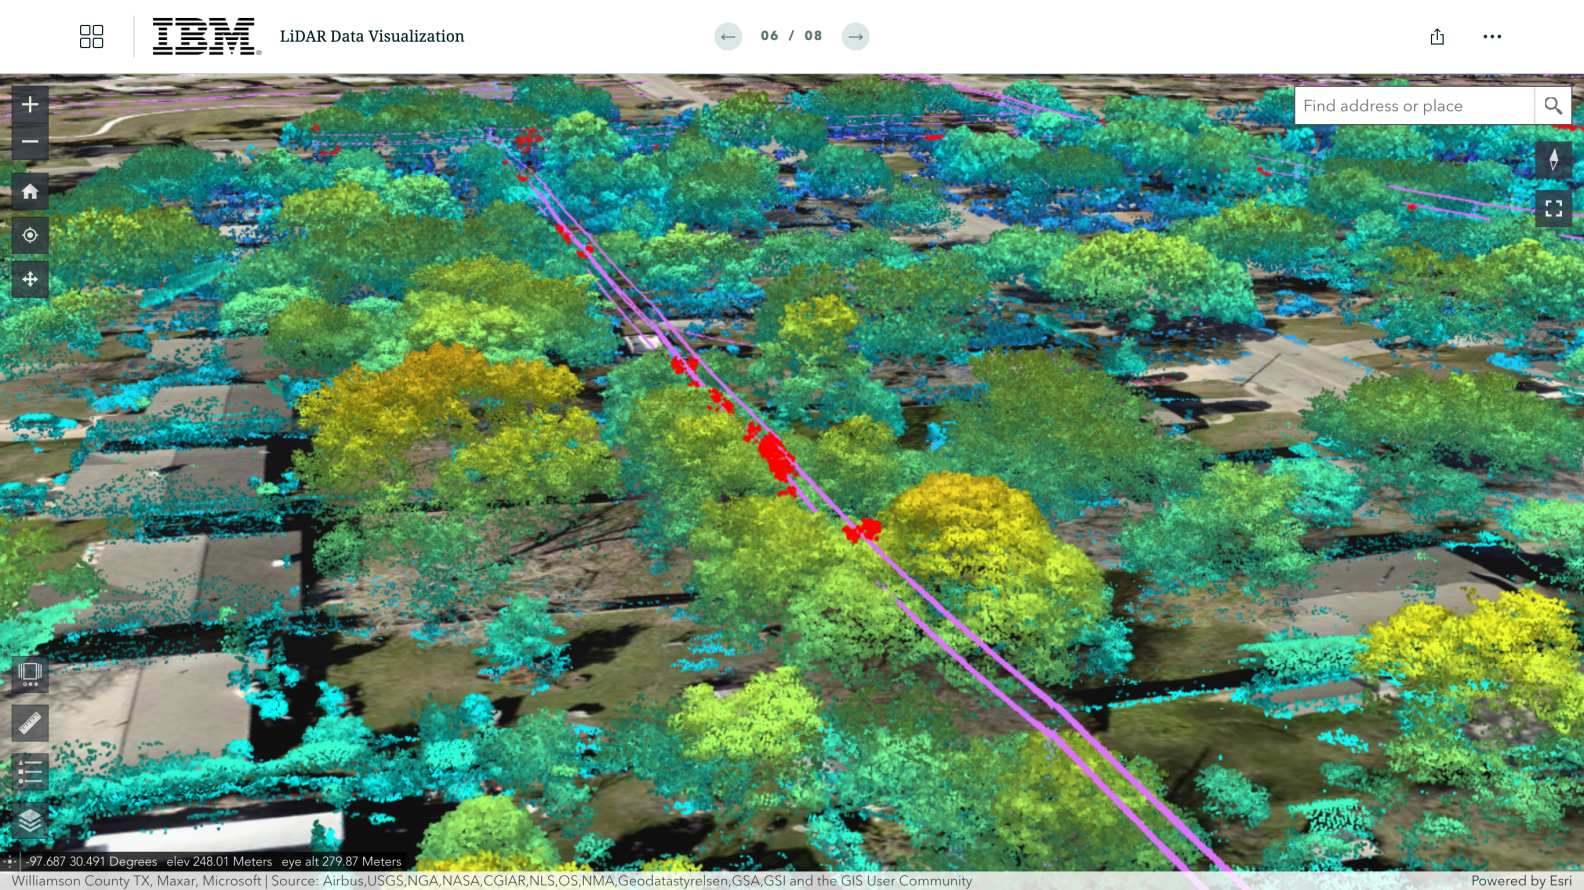
\includegraphics[scale = 0.2]{diagram9.png}
	\caption{LiDAR Technology \cite{IBM}}
	\label{fig:lidar}
\end{figure}

\end{itemize}

Moreover, with the advancement of technology, now anyone can contribute to the data of online maps, like Google Maps. Users can add panoramic street images using 360-degree cameras, enriching the maps with detailed visual representations of locations. Additionally, drone photography allows for the capture of unique aerial images, aiding in the update and refinement of maps in hard-to-reach or rapidly changing areas. These methods expand the capabilities of geographic data collection, making maps more accurate and informative.

\subsection {Transition from Multiplicity to Unity} \label{data:integrating}
The process of integrating GIS data into a unified view displayed in online maps like Google Maps requires complex conversion and synchronization of data from multiple sources \cite{Demers2008}:

\begin{enumerate}
\item \textbf{Converting Formats:} Different GIS data sources may have different formats. Digitalization converts paper maps and documents into digital formats. Vectorization converts raster images into vector data, allowing for more accurate processing and integration of information.

\item \textbf{Standardization and Synchronization:} Data are normalized to a common scale, projection and coordinate system. This ensures their compatibility and allows data from different sources to be combined into one consistent map.

\item \textbf{Merging and Visualization:} Different data layers such as topography, weather conditions, road networks and demographic information are merged to create layered maps. Once integrated, the data is visualized in a user-friendly way, providing an interactive and informative online map experience.

\item \textbf{Updating and Monitoring:} Online maps are updated regularly to reflect changes in geographic information. This requires constant monitoring and updating of data, which is achieved through automated data collection and integration systems.
\end{enumerate}

Consequently, the complex process of integrating GIS data allows users of online maps to obtain relevant, accurate and comprehensive information about the area in a user-friendly and understandable way.

\paragraph{Reaction to the Technology and People Topic:}
I believe that online maps play an inestimable role in helping people on a routine level. They provide us with reliable and relevant location data, allowing us to navigate, find places we need to go, and even estimate travel time. These amazing tools help us navigate in a city or in a foreign country, making our journeys more comfortable and safer.
\\From another point of view, I would like to point out that people also play an important role in updating online map data. A lot of users contribute by reporting changes in road infrastructure, new landmarks or current traffic situations. This collaboration between people and technology helps to keep the data on maps relevant and accurate, making them more useful and reliable for everyone. In this way, maps and people work together to create an amazing symbiosis that simplifies our daily activities in this life. 

\section{The Future of Online Mapping} \label{future}
Online maps are now an essential tool in our daily lives, having a significant impact on how we explore and interact with the world around us. As technology advances, they continue to evolve, offering more advanced and integrated solutions. These innovations open up new opportunities for improved navigation, which we'll explore next.

\subsection{Integration of AR Technologies} \label {future:ar}
The integration of augmented reality (AR) technologies into online maps opens a new chapter in the history of digital navigation and mapping. This merging offers the perspective of deep immersion, changing the way we interact with maps \cite{Bobrich2002}. 
\\At its core, AR technology allows navigation pointers and information to be overlaid directly onto real-world objects seen through a smartphone screen or AR glasses. This provides a more intuitive understanding of routes, especially in complex urban environments. And, for example, more and more of the world's IT companies are already starting to present their developed glasses and VR headsets with the ability to support real-time overlaying of computer-generated images on the surrounding world. Among such campaigns are Apple with its interesting Apple Vision Pro concept (Figure~\ref{fig:apple}) and Meta with its popular Meta Quest 3 model. So the market for AR devices is not standing still, pushing the integration of mapping services around the world.

\begin{figure}[h]
	\centering
	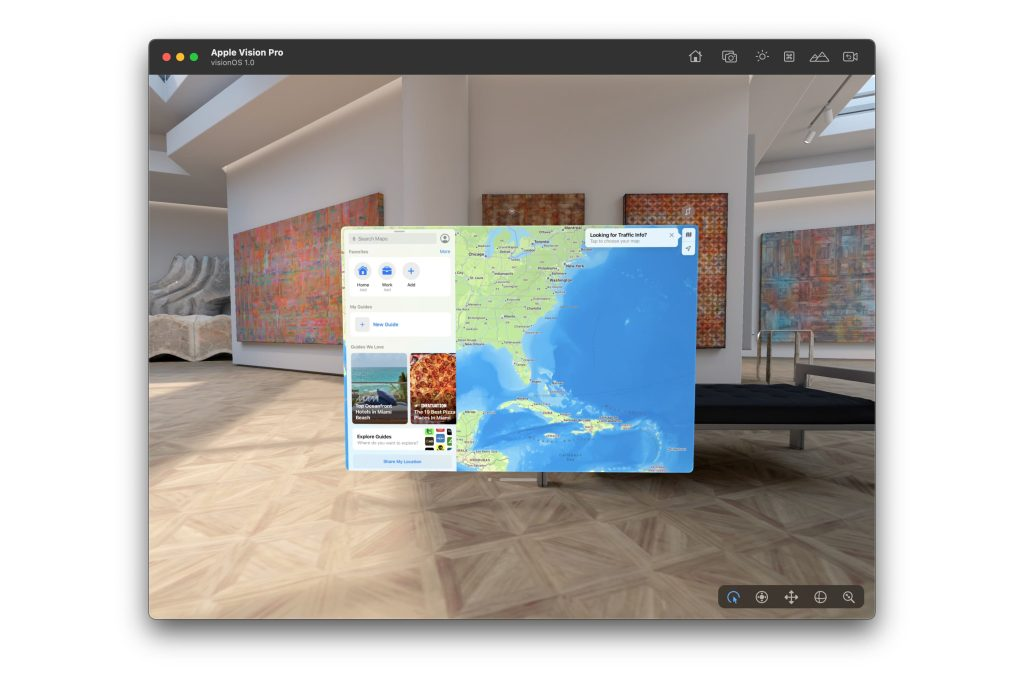
\includegraphics[scale = 0.37]{diagram7.jpg}
	\caption{How Maps will look through Apple Vision Pro \cite{Zelbo2023}}
	\label{fig:apple}
\end{figure}

Users can also get detailed information about the places they look at, including historical information, restaurant or shopping reviews, public transportation schedules and more, simply by pointing their devices at objects. Travelers can use AR maps to enrich their experience by getting interactive information about attractions, routes, and cultural features of the places they visit. And an interesting feature could be the ability to display what a place looked like in the past or how it will look in the future after planned changes or construction.
\\Integrating augmented reality (AR) technologies into online maps doesn't just add new functionality - it radically transforms the very essence of mapping. AR provides a deeper and more visually immersive experience, making maps not just navigation tools, but powerful means of interacting with the world around us.

\subsection{Integration into Self-Driving Vehicles} \label{future:vehicles}
Self-driving vehicles represent one of the most promising areas of development in modern transportation systems. Online maps play a key role in this process, as they provide autonomous vehicles with the data they need to navigate and make decisions on the road.
\\Google's self-driving cars \cite{NovakSelfDriving} show how online maps and LiDAR sensors integrate to create safe and efficient autonomous transportation. These vehicles use Google Maps data to provide information on road conditions, speed limits, and upcoming intersections, while sensors provide information on current traffic conditions. This synergy of technologies helps improve road safety, reduce accidents and make life easier for people who, for various reasons, cannot drive.
\\In the same way, the integration of online maps with the Internet of Things (IoT) represents a significant step in the evolution of digital navigation and urban infrastructure management. IoT devices scattered around the city, such as sensors on roads, traffic lights and parking lots, provide real-time data. This allows maps to display current traffic conditions, available parking spaces, and more. 
\\This is how IoT allows maps to help with traffic management by analyzing traffic congestion data and suggesting alternative routes to relieve traffic flow. And collecting data on traffic conditions, weather and other factors allows maps to not only display current conditions, but also predict future changes, such as worsening weather conditions or increased traffic congestion.

\subsection{Integrating AI to Create Map Data} \label{future:ai}
In today's world, artificial intelligence (AI) technologies are advancing at an unprecedented rate, opening new horizons in many fields. One of the significant advances of AI is its ability to generate images based on textual descriptions provided by the user.
\\It is this capability that gave rise to the idea of using AI as a tool for generating map data. Initially, this seemed like a promising approach: using AI to create maps could speed up the mapping process, making it more flexible and accessible. This approach not only implied time and resource savings, but also the ability to quickly adapt to changes in the environment, such as the construction of new roads or changes in the landscape.
\\However, the research conducted by the team of scientists focuses on the ethical aspects of using Artificial Intelligence (AI) in cartography, with a particular focus on map generation using DALL-E 2 \cite{Kang2023}. 
\\So, on the one hand, the use of AI can greatly speed up the map generation process. However, there are a number of ethical issues associated with the use of AI in cartography. For example, one of the main problems has been the inaccuracies observed in AI-generated maps, such as unclear and distorted boundaries between different regions. The shape of places could also be inconsistent and different in different generated maps. Another problem was pseudowords, symbols or signs that resemble country or city names, potentially leading to confusion or misinterpretation. In addition, AI-generated maps may contain fake countries, states/provinces, or counties that do not actually exist. These features could potentially lead to the spread of misinformation that could distort the public's perceptions of reality and have undesirable consequences (Figure~\ref{fig:ai}).

\begin{figure}[h]
	\centering
	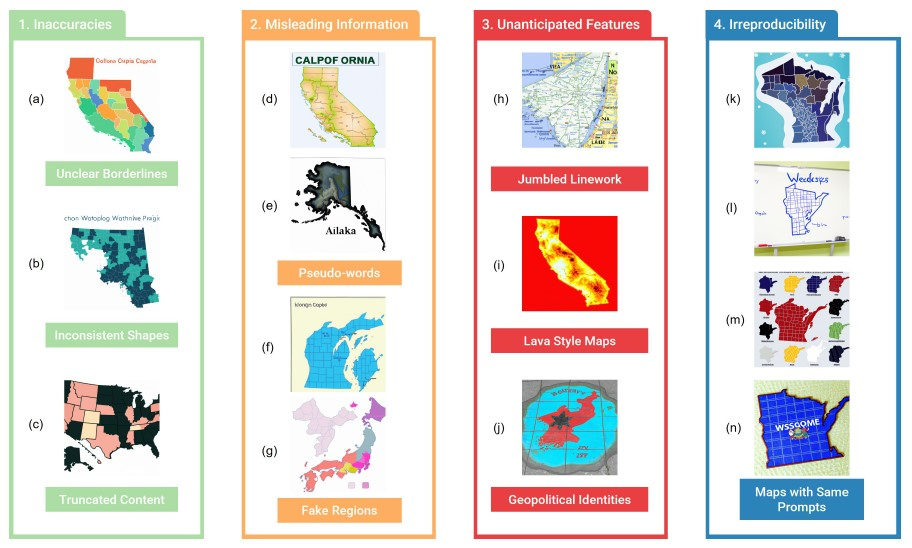
\includegraphics[scale = 0.6]{diagram8.jpg}
	\caption{Examples of AI-generated Map's Issues \cite{Kang2023}}
	\label{fig:ai}
\end{figure}

Therefore, researchers have developed an AI-generated map detector based on deep learning that is capable of identifying AI-generated maps. This can help in creating trusted maps and preventing the spread of misinformation created using AI-generated maps.
\\But don't forget that AI is capable of processing very large amounts of data very quickly. So AI analyzes data from satellites, aerial photos, and even information from users to update and refine maps. This includes changes in the landscape, new road configurations, and even temporary changes such as construction work.

\subsection{Perspectives} \label{future:perspectives}
In the future, thanks to technological innovation, online maps will become more intuitive, feature-rich, and personalized. However, this progressive development will also bring with it challenges related to data accuracy, privacy concerns, and ethical issues. Overall, the evolution of online maps will improve navigation and interactivity, but will require careful consideration of emerging challenges and risks.

\paragraph{Reaction to the Sustainability and Ethics Topic:}
Sustainability and ethics play an important role in the context of online maps and global interactive platforms. In today's world, there are a huge number of online maps used for navigation, travel, as well as in business and entertainment. However, when creating and using them, attention must be paid to sustainability in order to minimize the negative impact on the environment. This includes the use of efficient algorithms, which I discussed in Part ~\ref{internal}, that can reduce the power usage of the devices and reduce carbon emissions when using online maps.
\\From another perspective, ethics plays an important role in collecting and processing data to create online maps. Operators of such maps must be transparent and respect the privacy of users, as well as provide data security and confidentiality. In the case of artificial intelligence-generated maps, there are questions about the quality of such data. Incorrect use of data or privacy violations can cause serious ethical issues and negatively affect user's trust. Therefore, considering such aspects should be an integral part of the development and use of online maps to ensure their long-term and correct existence in today's world.


\section{Conclusion} \label{conclusion}
During the exploration, we delved deeper into understanding how online maps have transitioned from simple navigational aids to complex platforms that intertwine technology, data, and user experience. These maps are not just representations of our world but have become dynamic interfaces that profoundly connect us with our surroundings, constantly opening new horizons for interaction and comprehension.
\\Initially, as noted at the outset of our article, online maps were developed to satisfy basic navigational needs. However, as our analysis reveals, they have evolved into multifunctional platforms underpinned by complex algorithms and cutting-edge technologies. This transformation was made possible through the amalgamation of extensive data, including satellite imagery, geolocation information, and user interaction data.
\\Throughout the development of online maps, the integration of various technologies has been a key aspect. For instance, the use of geocoding and GPS technologies has significantly enhanced the accuracy and utility of maps for end-users. Maps have evolved from static images to interactive tools that enable users to not only find locations but also receive real-time information on traffic, weather, and other crucial aspects.
\\Modern online maps also reflect significant advancements in data analysis and processing. The development of artificial intelligence and machine learning has introduced new possibilities in interpreting and utilizing geospatial data. Thus, they provide not just location information but also assist in route planning, considering current road conditions and user preferences.
\\Recognizing this evolution brings us to a pivotal point in our research: the importance of balancing innovation with responsibility. The development of online maps should not lead to a complication of our world perception or create new issues for users. Instead, the aim is to make these tools facilitate human interaction with the environment, making it more comprehensible and accessible.
\\In conclusion, as we continue to develop and enhance online maps, we must strive to create tools that are not only technologically advanced but also user-friendly, safe, and beneficial to society. Such innovations have the potential to positively impact our daily lives, enriching our experience and expanding our capabilities to understand and explore the world around us. But even now, when the average person needs to find a route to a desired destination, many complex algorithms come into play. And ability of online maps to offer detailed and accurate navigation solutions is a direct result of their technological and functional development.

\bibliography{literatura}
\bibliographystyle{plain}

\end{document}
